\documentclass[a4paper,12pt]{article}
\usepackage[utf8]{inputenc}
\usepackage{amsmath}
\usepackage{amsfonts}
\usepackage{amssymb}
\usepackage{graphicx}
\usepackage{caption}
\usepackage{subcaption}
\usepackage{float}
\usepackage{siunitx}
\usepackage{booktabs}
\usepackage{hyperref}

\title{Reticolo}
\author{Francesco Giuseppe Minisini, Mattia Monzani, Gabriele Turi}
\date{\today}

\begin{document}

\maketitle
\hrule
\vspace{9pt}
\begin{abstract}
\noindent
In questa relazione viene documentata la misurazione degli indici di rifrazione di un prisma a base triangolare relativi a varie lunghezze d'onda e la verifica della relazione di Cauchy. La procedura sperimentale richiede, per la messa a punto dell'apparato, la misurazione della posizione angolare centrale \(\theta_0 = (58.783 \pm 0.010)^\circ\) e dell'angolo al vertice del prisma \(\alpha = (60.06 \pm 0.06)^\circ\). Conclusa la configurazione dell'apparato, sono stati misurati gli angoli di deviazione minima \(\delta_{\text{Min}}\) di sette righe dello spettro di emissione di una lampada ai vapori di mercurio, come riportato in Tabella \ref{tab:angoli_deviazione_minima}. Gli indicidi rifrazione associati sono stati calcolati in funzione della lunghezza d'onda, ottenendo i seguenti valori: \(n_{\text{Giallo 1}} = (1.7844 \pm 0.001)\),\(n_{\text{Giallo 2}} = (1.7849 \pm 00017)\),\(n_{\text{Verde}} = (1.7904 \pm 00017)\),\(n_{\text{Azzurro}} = (1.8033 \pm 00017)\),\(n_{\text{Indaco}} = (1.8234 \pm 0.001)\),\(n_{\text{Violetto 1}} = (1.8381 \pm 0.0017)\),\(n_{\text{Violetto 2}} = (1.8401 \pm 0.0017)\).
Infine, è stata verificata la relazione di Cauchy, ottenendo le costanti \(a = (2.992 \pm 0.008)\) e \(b = (6.41 \pm 0.19) \times 10^{-14} \, \text{m}^2\), con una compatibilità del \(97\%\) secondo il test del \(\chi^2\), testimoniando un buon accordo con il modello teorico.
\vspace{20pt}
\hrule
\end{abstract}
\vspace{2 pt}

\section{Messa a punto dell'apparato sperimentale}

\begin{figure}[H]
    \centering
    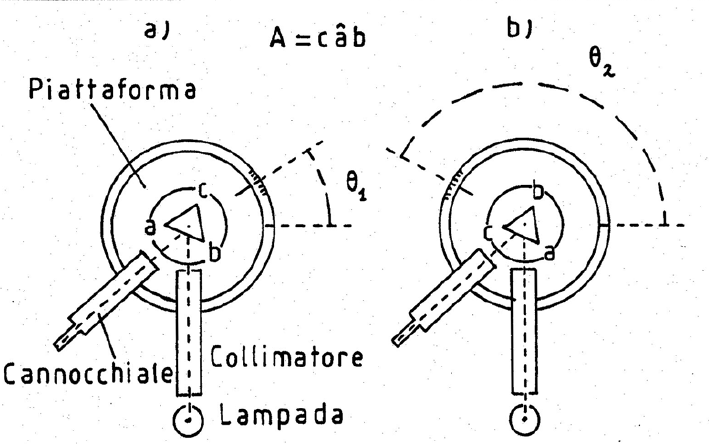
\includegraphics[width=0.6\textwidth]{apparato.png}
    \caption{Apparato sperimentale}
    \label{fig:camera_millikan}
\end{figure}

Lo spettrometro a prisma è uno strumento utilizzato per determinare le lunghezze d’onda di una luce non monocromatica. Si articola in: 
\begin{itemize}
    \item Un collimatore che viene posto davanti alla sorgente luminosa e che rende il fascio parallelo. 
    \item Un cannocchiale attraverso cui è possibile osservare le frange luminose. 
    \item Un prisma a base triangolare, posizionato e fissato sopra un sostegno. 
\end{itemize}
Prima di procedere con le misurazioni è necessario regolare l’apertura del collimatore per avere un fascio di luce parallela. Per fare ciò si posiziona lo strumento in un luogo dove è possibile mettere a fuoco un oggetto posto a grande distanza. Operando sulla rotella del cannocchiale si mette a fuoco l’oggetto. Insieme all'oggetto lontano si mette a fuoco anche il crocifilo con l'apposita regolazione, utilizzato per centrare le linee dello spettro in oggetto, assicurando una maggiore precisione delle misurazioni. In questo modo si assume che i raggi incidenti siano paralleli. La posizione della rotella del cannocchiale non verrà più variata nel corso dell’esperienza.  
Si posiziona ora la sorgente di luce dietro al collimatore e il cannocchiale davanti ad esso, in modo che guardando nel cannocchiale sia possibile osservare una linea luminosa. Ruotando la rotella del collimatore si mette a fuoco la linea e si cerca di renderla abbastanza fine, per avere misure più precise, ma non eccessivamente, poiché si rischia di non riuscire ad osservare la luce diffratta ad ordini più alti.  
Dopo aver posizionato il reticolo sull’apposito supporto, è possibile procedere con la misurazione della posizione angolare iniziale e successivamente dell'angolo al vertice del prisma, come descritto nel paragrafo \ref{sec:angolo al vertice}.

\section{Precisazioni sulle misurazioni angolari}
Ogni misurazione angolare è stata presa tramite il nonio integrato nell’apparato fornito in dotazione, che consente di leggere gli angoli in gradi sessagesimali (ovvero con i sottomultipli del grado che sono rappresentati dai primi). Dunque, ogni angolo misurato tramite il nonio è stato convertito in gradi sessadecimali, esprimendo i gradi in forma decimale convertendo i primi in frazioni decimali di grado, tramite divisione per 60 dei valori misurati in primi, siccome un primo equivale ad un sessantesimo di grado. Con la stessa conversione, le incertezze sulle misurazioni degli angoli, stabilite in primi, sono state trasformate in gradi. Eventualmente, i valori angolari misurati e calcolati, così come le loro incertezze, nell’esperimento sono stati convertiti in radianti (ciò per via dell’accettazione di angoli espressi in radianti da parte dei calcolatori impiegati nel calcolo delle funzioni
\[
\frac{\theta (^\circ)}{360^\circ} = \frac{\theta (\text{rad})}{2\pi},
\]
da cui:
\[
\theta (\text{rad}) = \frac{\theta (^\circ)}{360^\circ} \cdot 2\pi.
\]

\section{Misurazione dell’angolo al vertice del prisma}
\label{sec:angolo al vertice}
Il primo parametro fondamentale da misurare nella conduzione dell’esperimento di determinazione dell’indice di rifrazione della luce al variare della sua lunghezza d’onda è l’angolo al vertice del prisma a base triangolare, impiegato per studiare la dispersione cromatica della luce attraverso il fenomeno della rifrazione di essa attraverso il prisma. Per condurre questa prima misurazione è possibile orientare il canocchiale della piattaforma di lavoro in modo che sia visibile attraverso di esso la riga di luce emessa dalla lampada utilizzata e riflessa dalla faccia del prisma che posizioniamo sulla piattaforma, assicurandosi di centrare la riga con il crocifilo visibile nel cannocchiale. In seguito, si procederà nel ruotare la piattaforma, e quindi l’orientazione nello spazio del prisma, variando dunque l’angolo di incidenza e di conseguenza quello di riflessione della luce che impatta sul prisma, fino a quando non si riverifica la condizione secondo cui la riga verticale luminosa emessa dalla lampada risulterà nuovamente in corrispondenza del crocifilo (si noti come il cannocchiale nel mentre debba essere lasciato fermo). Si può notare, attraverso una semplice schematizzazione geometrica della situazione, che l’angolo al vertice del prisma è ottenibile sottraendo all’angolo piatto, di \( 180^\circ \), il valore dell’angolo di cui si è dovuto ruotare la piattaforma e dunque il prisma nella procedura appena esposta.(magari inserire immagine).Dunque, per determinare l’angolo al vertice \( \alpha \) del prisma è sufficiente:
\begin{itemize}
    \item Misurare la posizione angolare iniziale \( \theta_1 \) della piattaforma al momento della visualizzazione attraverso di esso per riflessione sul prisma della luce della lampada.
    \item Ruotare la piattaforma fino a quando la riga luminosa non ritornerà ad essere visibile sul crocifilo del cannocchiale e misurare in questa situazione la posizione angolare finale \( \theta_2 \) della piattaforma, in modo da calcolare lo spostamento angolare \( \Delta\theta \) applicato alla piattaforma, tramite differenza delle due posizioni angolari:
\end{itemize}
\[
\Delta\theta = |\theta_2 - \theta_1|.
\]
A quel punto l’angolo \( \alpha \) al vertice del prisma si determina con il calcolo:
\[
\alpha(^\circ) = |180^\circ - \Delta\theta(^\circ)|.
\]
L’incertezza su una misura dell’angolo al vertice del prisma è di conseguenza uguale all’incertezza sullo spostamento angolare della piattaforma:
\[
\sigma_\alpha = \sigma_{\Delta\theta} = \sqrt{(\sigma_{\theta_1})^2 + (\sigma_{\theta_2})^2}.
\]

Come incertezza sulle misurazioni angolari (misurazioni che sono state tutte riportate al primo, nonostante il nonio impiegato apprezzi anche i mezzi primi, per questioni di difficoltà di lettura delle tacche) condotte durante tutto l’esperimento si è scelta un’incertezza di 2 primi di grado, stimata ragionevolmente considerando le difficoltà di visibilità nella lettura del nonio angolare usato per le misurazioni. 
Iterando queste misurazioni per 6 volte si sono determinati 6 valori per \( \alpha \), di cui si è ottenuta la miglior stima tramite media aritmetica. L’incertezza finale su \( \alpha \) è stata stimata statisticamente tramite il calcolo della deviazione standard della media delle 6 misurazioni ottenute.
Dunque, \( \alpha \) è risultato pari a:
\[\alpha = (60.06 \pm 0.06)^\circ.\] 

\section{Misurazioni angoli di deviazione minima}
Siccome da questo momento in poi dell’esperimento ogni misurazione angolare misurata verrà considerata rispetto alla direzione normale alla lampada di emissione della luce, è essenziale procedere subito con la misurazione della posizione angolare della direzione centrale, modo da esprimere ogni posizione angolare misurata tramite differenza del valore angolare misurato rispetto al valore della posizione angolare centrale.
Dunque, si sono misurati col nonio 6 valori della posizione angolare centrale \( \theta_0 \), assegnando ogni volta al valore di \( \theta_0 \) il valore della posizione in cui si trova il cannocchiale nel caso in cui la riga centrale emessa dalla sorgente luminosa si trovi in corrispondenza del crocifilo, di cui si è eseguita la media aritmetica per fornire una miglior stima e la deviazione standard della media per esibire un’incertezza, ottenendo:
\[
\theta_0 = (58.783 \pm 0.010)^\circ
\]
La direzione centrale individuata dalla posizione angolare \( \theta_0 \) è quella lungo cui la luce emessa dalla lampada si propaga se non subisce deviazioni.
A causa della rifrazione causata dall’attraversamento del prisma, la riga luminosa emessa dalla lampada (nella fattispecie si è utilizzata una lampada ai vapori di mercurio) subisce il fenomeno della dispersione cromatica, che permette di visualizzare con il cannocchiale le righe dello spettro di emissione del mercurio a posizioni angolari differenti in base alla lunghezza d’onda del colore.
È possibile dimostrare e osservare come, variando l’orientazione del prisma, si vari l’angolo di deviazione di ciascuna lunghezza d’onda, fino ad una condizione di deviazione minima per un’opportuna orientazione del prisma.
È possibile configurare il sistema in modo che si abbia questa condizione di deviazione minima delle righe dello spettro di emissione ruotando la piattaforma del prisma, osservando di conseguenza dal cannocchiale lo spostamento delle righe di emissione, fino a quando non si giunge alla condizione limite in cui si osserva l’inversione del senso di spostamento delle righe.
Ponendo il sistema in questa condizione limite, è possibile, centrando ognuna delle righe con il crocifilo del cannocchiale, misurare l’angolo di deviazione minima di ognuna di esse, misurando con il nonio la loro posizione angolare e calcolando la differenza con la posizione angolare centrale \( \theta_0 \):
\[
\delta_{\text{Min}} = |\theta_{\text{Min}} - \theta_0|
\]
L’incertezza \( \sigma_{\delta_{\text{Min}}} \) su \( \delta_{\text{Min}} \) è quindi determinabile attraverso il calcolo:
\[
\sigma_{\delta_{\text{Min}}} = \sqrt{(\sigma_{\theta_0})^2 + (\sigma_{\theta_{\text{Min}}})^2}
\]
Per ogni lunghezza d’onda dello spettro di emissione del mercurio sono stati calcolati 5 valori di \( \delta_{\text{Min}} \), di cui si è estratta la media e la deviazione standard della media.
Di seguito i colori delle righe dello spettro di emissione del mercurio che è stato possibile osservare, le loro lunghezze d’onda (note, con incertezza trascurabile), e i rispettivi angoli di deviazione minima misurati tramite il procedimento sopra indicato:

\begin{table}[H]
    \centering
    \begin{tabular}{ccc}
    \hline
    \textbf{Colore} & \textbf{\( \lambda \)} & \textbf{\( \delta_{\text{Min}} \)} \\ \hline
    Giallo 1 & \( 5790 \, \text{\AA} \) & \( (66.4600 \pm 0.0018)^\circ \) \\ 
    Giallo 2 & \( 5770 \, \text{\AA} \) & \( (66.527 \pm 0.003)^\circ \) \\ 
    Verde & \( 5461 \, \text{\AA} \) & \( (67.230 \pm 0.004)^\circ \) \\ 
    Azzurro & \( 4960 \, \text{\AA} \) & \( (68.917 \pm 0.008)^\circ \) \\ 
    Indaco & \( 4358 \, \text{\AA} \) & \( (71.6633 \pm 0.0028)^\circ \) \\ 
    Violetto 1 & \( 4077 \, \text{\AA} \) & \( (73.773 \pm 0.006)^\circ \) \\ 
    Violetto 2 & \( 4047 \, \text{\AA} \) & \( (74.057 \pm 0.004)^\circ \) \\ \hline
    \end{tabular}
    \caption{Angoli di deviazione minima per le righe dello spettro di emissione del mercurio.}
    \label{tab:angoli_deviazione_minima}
\end{table}
    
\section{Calcolo degli indici di rifrazione}

Attraverso considerazioni di carattere geometrico e l’utilizzo del calcolo differenziale è possibile dimostrare la seguente relazione:
\[
n(\lambda) = \frac{\sin\left(\frac{\alpha + \delta_{\text{Min}}(\lambda)}{2}\right)}{\sin\left(\frac{\alpha}{2}\right)}
\]
Dunque, è possibile calcolare l’indice di rifrazione \( n(\lambda) \) di ogni lunghezza d’onda nel vetro che compone il prisma, a partire dal valore \( \alpha \) dell’angolo al vertice del prisma e dal valore dell’angolo di deviazione minima \( \delta_{\text{Min}}(\lambda) \) della lunghezza d’onda di interesse \( \lambda \).
L’incertezza sull’indice di rifrazione è ottenibile mediante la propagazione dell’errore sviluppando il calcolo:
\[
\sigma_n = \sqrt{\left( \frac{\partial n}{\partial \alpha} \sigma_\alpha \right)^2 + \left( \frac{\partial n}{\partial \delta_{\text{Min}}} \sigma_{\delta_{\text{Min}}} \right)^2 }
\]
Di seguito sono riportati i valori dell’indice di rifrazione associati ad ogni lunghezza d’onda dello spettro di emissione del mercurio:

\begin{table}[H]
\centering
\begin{tabular}{ccc}
\hline
\textbf{Colore} & \textbf{\( \lambda \)} & \textbf{\( n \)} \\ \hline
Giallo 1 & \( 5790 \, \text{\AA} \) & \( 1.7844 \pm 0.0017 \) \\ 
Giallo 2 & \( 5770 \, \text{\AA} \) & \( 1.7849 \pm 0.0017 \) \\
Verde & \( 5461 \, \text{\AA} \) & \( 1.7904 \pm 0.0017 \) \\ 
Azzurro  & \( 4960 \, \text{\AA} \) & \( 1.8033 \pm 0.0017 \) \\ 
Indaco & \( 4358 \, \text{\AA} \) & \( 1.8234 \pm 0.0017 \) \\ 
Violetto 1 & \( 4077 \, \text{\AA} \) & \( 1.8381 \pm 0.0017 \) \\ 
Violetto 2 & \( 4047 \, \text{\AA} \) & \( 1.8401 \pm 0.0017 \) \\ \hline
\end{tabular}
\caption{Indici di rifrazione calcolati per le diverse lunghezze d’onda dello spettro di emissione del mercurio.}
\label{tab:indici_rifrazione}
\end{table}

\section{Verifica della relazione di Cauchy}
L’obiettivo finale dell’esperimento consiste nel descrivere come varia l’indice di rifrazione della luce di un dato colore al variare della lunghezza d’onda del colore. 
È possibile dimostrare come secondo l’indice di rifrazione della luce in un mezzo dipenda dalla lunghezza d’onda della luce tramite la cosiddetta “relazione di Cauchy”:
\[
n^2(\lambda) = a + \frac{b}{\lambda^2}
\]
Dove \( a \) e \( b \) sono delle costanti. In particolare, \( a \) è un numero reale dimensionale e \( b \) è misurabile in \( \text{m}^2 \). 
Sia ora \( Y(X) \equiv n^2 \) e sia \( X \equiv \frac{1}{\lambda^2} \).
Per valutare la validità della relazione e calcolare le due costanti a partire dai dati raccolti è stata eseguita una regressione lineare utilizzando il metodo dei “minimi quadrati”, in modo da determinare la retta di equazione:
\[
Y = a + bX
\]
che, minimizzando la quantità definita come \( \chi^2 \), meglio sia adatta alle 7 coppie di punti sperimentali \( (X, Y) = \left(\frac{1}{\lambda^2}, n^2\right) \) ottenute dalle misurazioni e dai calcoli.
\[
a = 2.992 \pm 0.008
\]
\[
b = (6.41 \pm 0.19) \times 10^{-14} \, \text{m}^2
\]

Il test del \( \chi^2 \) restituisce un accordo del \( 97 \% \), rappresentando un risultato ampiamente soddisfacente.

\begin{figure}[H]
    \centering
    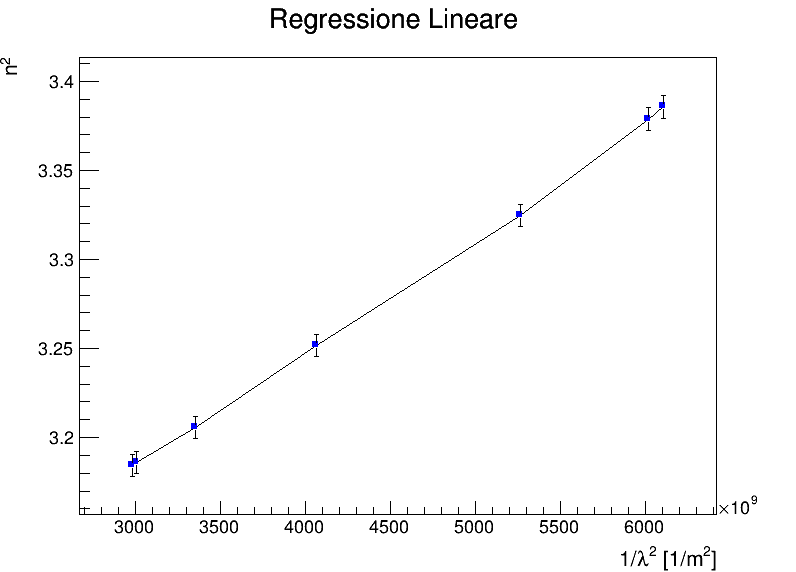
\includegraphics[width=0.7\textwidth]{image.png}
    \caption{Regressione lineare ottenuta}
    \label{fig:regressione}
\end{figure}

L’incertezza sulla quantità \( Y = n^2 \) è ottenibile mediante propagazione dell’errore tramite il calcolo:
\[
\sigma_Y = 2n \sigma_n
\]
L’incertezza sull’ascissa \( X = \frac{1}{\lambda^2} \) è ritenibile trascurabile, in quanto viene ritenuta trascurabile l’incertezza su \( \lambda \), dal momento che i valori delle lunghezze d’onda sono stati forniti.


\end{document}